\documentclass[12pt]{article}
\usepackage{amsmath}
\usepackage{amssymb}
\usepackage{cancel}
\usepackage{graphicx}
\usepackage{physics}
\usepackage{siunitx}
\usepackage{pgfplots}
\usepackage{wrapfig}

\AtBeginDocument{\RenewCommandCopy\qty\SI}
\newcommand{\E}[1]{\times 10^{#1}}

\title{
    Worksheet \#4
    \\  \small
    PHYS 4C: Waves and Thermodynamics
    }
\author{Donald Aingworth IV}
\date{September 15, 2025}

\begin{document}
    \DeclareSIUnit{\celsiusdegree}{C^\circ}
    \DeclareSIUnit{\atm}{ atm}

    \maketitle

    \section{Problem}
        A monatomic ideal gas expands from 3.0 l to 4.0 l along a process defined by\\
        \begin{tabular}[pos]{l c r}
            $P = a/V^2$  &$a = 10.0\,\unit{\atm}\ l^2$ &(l = liter)
        \end{tabular}\\
        The initial temperature of the ideal gas is 300 K.

        a. (2 points) Express 1 atm $l$ in terms of SI units.

        b. (4 points) Determine the initial and final pressure of the gas and sketch the process in a P-V diagram.

        c. (2 points) Calculate the number of molecules of the gas. How many moles does that correspond to?

        d. (2 points) Determine the final temperature of the gas.

        e. (2 points) Calculate the change in the internal energy of the gas.

        f. (4 points) Determine the net work done on/by the gas during this process.

        g. (4 points) Determine the net heat flow into / out of the gas during this process. 
        Does the direction of heat flow make sense? 
        (Compare the given process to adiabatic and isothermal processes.)

        \subsection{Solution (a)}
            We know the ratio of pascals to atm. 
            We can turn this from atmosphere liters squared to pascal liters squared.
            \begin{align}
                a   &=  1\,\unit{\atm\,\liter} * 1.01\E{5}\,\unit{\pascal/\atm}
                    =   1.01\E{5}\,\unit{\pascal\,\liter}\\
                    &=  1.01\E{5}\,\unit{\pascal\,\liter} \times \frac{10^{-3}\,\unit{\meter^3}}{1\,\unit{\liter}}
                    =   \boxed{1.01\E{2}\,\unit{\pascal\,\meter^3}}
            \end{align}

        \subsection{Solution (b)}
            The initial and final pressures can be calculated.
            \begin{align}
                P(V)    &=  \frac{a}{V^2}\\
                P_i =   P(3\,\unit{\liter}) &=  \frac{1.01\E{6}\,\unit{\pascal\,\liter^2}}{9\unit{\liter^2}}
                    =   1.122\E{5}\,\unit{\pascal}\\
                P_f =   P(4\,\unit{\liter}) &=  \frac{1.01\E{6}\,\unit{\pascal\,\liter^2}}{16\unit{\liter^2}}
                    =   6.3125\E{4}\,\unit{\pascal}
            \end{align}
            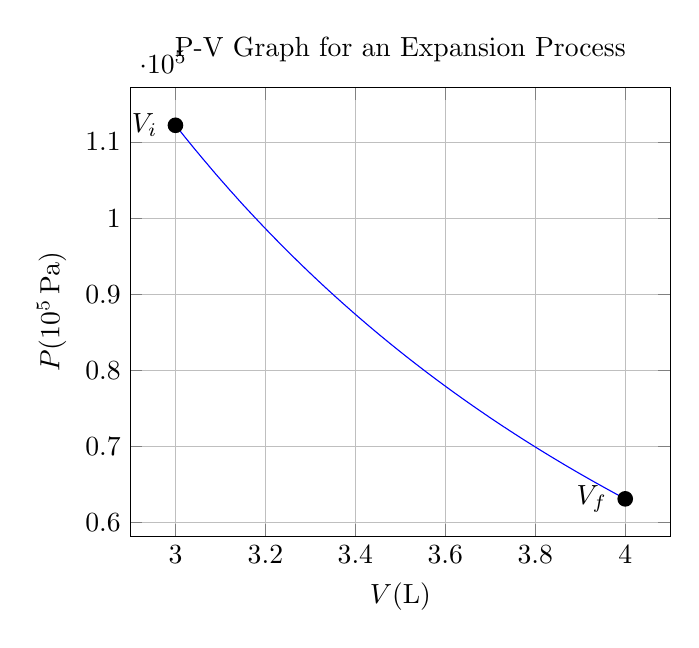
\begin{tikzpicture}
                \begin{axis}[
                    title={P-V Graph for an Expansion Process},
                    xlabel={$V (\unit{\liter})$},
                    ylabel={$P (10^5\,\unit{\pascal})$},
                    grid=major,
                ]
                    \addplot[domain=3:4, samples=100, blue] {1.01*10^6/x^2};
                    \node[label={180:{$V_i$}},circle,fill,inner sep=2pt] at (axis cs:3,1.122*10^5) {};
                    \node[label={180:{$V_f$}},circle,fill,inner sep=2pt] at (axis cs:4,6.3125*10^4) {};
                \end{axis}
            \end{tikzpicture} 

        \subsection{Solution (c)}
            We use the ideal gas law here on the initial conditions.
            \begin{gather}
                pV  =   NkT\\
                \begin{align}
                    N   &=  \frac{pV}{kT}
                        =   \frac{1.122\E{5}\,\unit{\pascal} * 3\E{-3}\,\unit{\meter^3}}{1.38\E{-23}\,\unit{\joule/\kelvin} * 300\,\unit{\kelvin}}\\
                        &=  8.13\E{22}\,\text{molecules}
                        =   \boxed{0.135\,\unit{\mole}}
                \end{align}
            \end{gather}

        \subsection{Solution (d)}
            We can again use the ideal gas law.
            \begin{align}
                pV  &=  NkT\\
                T   &=  \frac{pV}{Nk}
                    =   \frac{6.3125\E{4}\,\unit{\pascal} * 4\E{-3}\,\unit{\meter^3}}{8.13\E{22}\,\text{molecules} * 1.38\E{-23}\,\unit{\joule/\kelvin}}\\
                    &=  \boxed{225\unit{\kelvin}}
            \end{align}

        \subsection{Solution (e)}
            This gas is monatomic, so $\alpha = \frac{3}{2}$.
            \begin{align}
                \Delta E_{\rm int}  &=  \alpha Nk\,\Delta T\\
                    &=  \frac{3}{2} * 8.13\E{22}\,\text{molecules} * 1.38\E{-23}\,\unit{\joule/\kelvin} * (-75\unit{\kelvin})\\
                    &=  \boxed{-126.21825\,\unit{\joule}}
            \end{align}

        \subsection{Solution (f)}
            The work is determined by an integral.
            \begin{align}
                W   &=  -\int p\,dV
                    =   -\int_{3\,\unit{\liter}}^{4\,\unit{\liter}} \frac{a}{V^2}\,dV\\
                    &=  -a \left[ -\frac{1}{V} \right]_{3\,\unit{\liter}}^{4\,\unit{\liter}}
                    =   -a\left( \frac{1}{3} - \frac{1}{4} \right)\\
                    &=  -\frac{1.01\E{6}\,\unit{\pascal\,\liter^2}}{12\unit{\liter}}\\
                    &=  -8.4167\E{4}\,\unit{\pascal\,\liter} \times \frac{10^{-3}\,\unit{\meter^3}}{1\,\unit{\liter}}\\
                    &=  \boxed{-84.167\,\unit{\joule}}
            \end{align}

        \subsection{Solution (g)}
            The second law of thermodynamics is our friend today.
            \begin{gather}
                \Delta E_{\rm int}  =   Q + W\\
                \begin{align}
                    Q   &=  \Delta E_{\rm int} - W
                        =   -126.21825\,\unit{\joule} + 84.167\,\unit{\joule}
                        =   \boxed{-42.05\,\unit{\joule}}
                \end{align}
            \end{gather}

\end{document}